\chapter{Testing and Analysis}
\section{System Testing}
In this chapter, will be explain about testing and analysis that used in this final project. The result of this testing and analyzing process will show how good the perfomance of the system is. There are two aspects that will be the concern in this step, they are execution time and the correctness of the outputs.  

\subsection{Testing Objective}
Based on the system model in chapter 3, the shortest path algorithms will be implemented in Indoor Routing System using three dimensional data structure. And the objectives of this testing process are:
\begin{enumerate}
%	\item Knowing that the shortest path algorithms can be implemented in three dimensional graph data structure.
	\item To get the best system's performance by comparing the execution time between Dijkstra's, Bellman-Ford, Floyd-Warshall, and A* algorithms.
	\item To analyze Dijkstra's, Bellman-Ford, Floyd-Warshall, and A* algorithms by how it works, the output, and the time complexity.
	\item To get the system's accuracy by comparing and analyzing the distance as the result of TELUR IRIS system and  the distance in real life.
\end{enumerate}

\subsection{Testing Scenario}
The following statements are the scenario of testing process:

\begin{enumerate}
	\item \textbf{Testing of system's perfomance in execution time}. In this section, each of dijkstra's, bellman-ford, floyd-warshall, and A* will be tested five times to get the execution time. After that the average amount can be assumed as the exact execution time. this testing will be implemented in both open and close space wich is has different count of nodes and edges.
	
	\item \textbf{Testing of the shortest path algorithms.} In this section, each of dijkstra's, bellman-ford, floyd-warshall, and A* will be tested by its output, pseudocode, and time complexity. Each algorithm has different way of works. Time complexity could be obtained by analyzing the loop of the pseudocode.
	
	\item \textbf{Testing of system's accuracy}. In this section, comparison between the distance as the result of TELUR IRIS system and  the distance in real life will be calculated. For each scenario, there will be three samples of calculation result.
	
	The scenario of this test will be devided into 4, those are:
	\begin{itemize}
		\item Distance calculation between two rooms that have same Building\textunderscore{ID} and same $z$ attribute.
		\item Distance calculation between two rooms that have same Building\textunderscore{ID} but different $z$ attribute.
		\item Distance calculation between two rooms that have different Building\textunderscore{ID} but same $z$ attribute.
		\item Distance calculation between two rooms that have different Building\textunderscore{ID} and different $z$ attribute.
	\end{itemize}
	
\end{enumerate}

\section{Testing Result}

\subsection{Time Execution Testing}
Here are the result of time execution testing. For the testing sample, the shortest path between node IF1.01.01 to node IF3.03.07 were choosen as a sample. This test implemented Dijkstra, Floyd-Warshall, Bellman-Ford, and A* Algorithms to search that shortest path. The testing do the searching process five times for each algorithms and it took the average value of the execution times as the result. All the time values are in seconds. 
\\\\
\textbf{The output of five times Dijkstra's Algorithm running:}\\
*****dijkstra algorithm node IF1.01.01 to IF3.03.07*****\\
graph.getNodeCount() = 272\\
execution time dijkstra : 0.176570559\\
*****dijkstra algorithm node IF1.01.01 to IF3.03.07*****\\
graph.getNodeCount() = 266\\
execution time dijkstra\textunderscore{close} : 0.059495901\\
executed in 0.23606646 seconds\\
\\
*****dijkstra algorithm node IF1.01.01 to IF3.03.07*****\\
graph.getNodeCount() = 272\\
execution time dijkstra : 0.059805929\\
*****dijkstra algorithm node IF1.01.01 to IF3.03.07*****\\
graph.getNodeCount() = 266\\
execution time dijkstra\textunderscore{close} : 0.030269795\\
executed in 0.090075724 seconds\\
\\
*****dijkstra algorithm node IF1.01.01 to IF3.03.07*****\\
graph.getNodeCount() = 272\\
execution time dijkstra : 0.048037625\\
*****dijkstra algorithm node IF1.01.01 to IF3.03.07*****\\
graph.getNodeCount() = 266\\
execution time dijkstra\textunderscore{close} : 0.035783754\\
executed in 0.083821379 seconds\\
\\
*****dijkstra algorithm node IF1.01.01 to IF3.03.07*****\\
graph.getNodeCount() = 272\\
execution time dijkstra : 0.04465599\\
*****dijkstra algorithm node IF1.01.01 to IF3.03.07*****\\
graph.getNodeCount() = 266\\
execution time dijkstra\textunderscore{close} : 0.030038336\\
executed in 0.074694326 seconds\\
\\
*****dijkstra algorithm node IF1.01.01 to IF3.03.07*****\\
graph.getNodeCount() = 272\\
execution time dijkstra : 0.06649877\\
*****dijkstra algorithm node IF1.01.01 to IF3.03.07*****\\
graph.getNodeCount() = 266\\
execution time dijkstra\textunderscore{close} : 0.032153671\\
executed in 0.098652441 seconds\\
\\\\
\textbf{The output of five times Floyd-Warshall Algorithm running:}\\
*****Floyd-Warshal algorithm node IF1.01.01 to IF3.03.07*****\\
graph.getNodeCount() = 272\\
execution time fw : 0.280716078\\
*****Floyd-Warshal algorithm node IF1.01.01 to IF3.03.07*****\\
graph.getNodeCount() = 266\\
execution time fw\textunderscore{close} : 0.175645076\\
executed in 0.456361154 seconds\\
\\
*****Floyd-Warshal algorithm node IF1.01.01 to IF3.03.07*****\\
graph.getNodeCount() = 272\\
execution time fw : 0.262804205\\
*****Floyd-Warshal algorithm node IF1.01.01 to IF3.03.07*****\\
graph.getNodeCount() = 266\\
execution time fw\textunderscore{close} : 0.100703012\\
executed in 0.363507217 seconds\\
\\
*****Floyd-Warshal algorithm node IF1.01.01 to IF3.03.07*****\\
graph.getNodeCount() = 272\\
execution time fw : 0.295337272\\
*****Floyd-Warshal algorithm node IF1.01.01 to IF3.03.07*****\\
graph.getNodeCount() = 266\\
execution time fw\textunderscore{close} : 0.081183668\\
executed in 0.37652094 seconds\\
\\
*****Floyd-Warshal algorithm node IF1.01.01 to IF3.03.07*****\\
graph.getNodeCount() = 272\\
execution time fw : 0.283726813\\
*****Floyd-Warshal algorithm node IF1.01.01 to IF3.03.07*****\\
graph.getNodeCount() = 266\\
execution time fw\textunderscore{close} : 0.238191704\\
executed in 0.521918517 seconds\\
\\
*****Floyd-Warshal algorithm node IF1.01.01 to IF3.03.07*****\\
graph.getNodeCount() = 272\\
execution time fw : 0.282648442\\
*****Floyd-Warshal algorithm node IF1.01.01 to IF3.03.07*****\\
graph.getNodeCount() = 266\\
\\execution time fw\textunderscore{close} : 0.263365865
\\executed in 0.546014307 seconds
\\\\
\\\textbf{The output of five times Bellman-Ford Algorithm running:}
\\*****Bellman-Ford algorithm node IF1.01.01 to IF3.03.07*****
\\graph.getNodeCount() = 272
\\execution time bf : 0.337928182
\\*****Bellman-Ford algorithm node IF1.01.01 to IF3.03.07*****
\\graph.getNodeCount() = 266
\\execution time bf\textunderscore{close} : 0.188902291
\\executed in 0.526830473 seconds
\\
\\*****Bellman-Ford algorithm node IF1.01.01 to IF3.03.07*****
\\graph.getNodeCount() = 272
\\execution time bf : 0.221083213
\\*****Bellman-Ford algorithm node IF1.01.01 to IF3.03.07*****
\\graph.getNodeCount() = 266
\\execution time bf\textunderscore{close} : 0.234484116
\\executed in 0.455567329 seconds
\\
\\*****Bellman-Ford algorithm node IF1.01.01 to IF3.03.07*****
\\graph.getNodeCount() = 272
\\execution time bf : 0.29284962
\\*****Bellman-Ford algorithm node IF1.01.01 to IF3.03.07*****
\\graph.getNodeCount() = 266
\\execution time bf\textunderscore{close} : 0.240597956
\\executed in 0.533447576 seconds
\\
\\*****Bellman-Ford algorithm node IF1.01.01 to IF3.03.07*****
\\graph.getNodeCount() = 272
\\execution time bf : 0.273845218
\\*****Bellman-Ford algorithm node IF1.01.01 to IF3.03.07*****
\\graph.getNodeCount() = 266
\\execution time bf\textunderscore{close} : 0.246817972
\\executed in 0.52066319 seconds
\\
\\*****Bellman-Ford algorithm node IF1.01.01 to IF3.03.07*****
\\graph.getNodeCount() = 272
\\execution time bf : 0.28561423
\\*****Bellman-Ford algorithm node IF1.01.01 to IF3.03.07*****
\\graph.getNodeCount() = 266
\\execution time bf\textunderscore{close} : 0.236419664
\\executed in 0.522033894 seconds
\\\\
\\\textbf{The output of five times A* Algorithm running:}
\\*****A* algorithm node IF1.01.01 to IF3.03.07*****
\\graph.getNodeCount() = 272
\\execution time astar : 0.065852526
\\*****A* algorithm node IF1.01.01 to IF3.03.07*****
\\graph.getNodeCount() = 266
\\execution time astar\textunderscore{close} : 0.016076835
\\executed in 0.081929361 seconds
\\
\\*****A* algorithm node IF1.01.01 to IF3.03.07*****
\\graph.getNodeCount() = 272
\\execution time astar : 0.03272878
\\*****A* algorithm node IF1.01.01 to IF3.03.07*****
\\graph.getNodeCount() = 266
\\execution time astar\textunderscore{close} : 0.023422293
\\executed in 0.056151073 seconds
\\
\\*****A* algorithm node IF1.01.01 to IF3.03.07*****
\\graph.getNodeCount() = 272
\\execution time astar : 0.030558941
\\*****A* algorithm node IF1.01.01 to IF3.03.07*****
\\graph.getNodeCount() = 266
\\execution time astar\textunderscore{close} : 0.01713822
\\executed in 0.047697161 seconds
\\
\\*****A* algorithm node IF1.01.01 to IF3.03.07*****
\\graph.getNodeCount() = 272
\\execution time astar : 0.026007271
\\*****A* algorithm node IF1.01.01 to IF3.03.07*****
\\graph.getNodeCount() = 266
\\execution time astar\textunderscore{close} : 0.022123787
\\executed in 0.048131058 seconds
\\
\\*****A* algorithm node IF1.01.01 to IF3.03.07*****
\\graph.getNodeCount() = 272
\\execution time astar : 0.036428937
\\*****A* algorithm node IF1.01.01 to IF3.03.07*****
\\graph.getNodeCount() = 266
\\execution time astar\textunderscore{close} : 0.032021663
\\executed in 0.0684506 seconds
\\\\

The tables below shows the comparison clearly according to the console output of the system above. Table \ref{table:2} shows the comparison of the shortest path algorithms in showing the actual shortest path where all nodes (total 272 nodes) of the graph are included in the algorithm's calculation. Table \ref{table:3} shows the comparison of the shortest path algorithms in showing the shortest path in close space where nodes wich are the open space will not be calculated in shortest path algorithm (total 266 nodes).


% Please add the following required packages to your document preamble:
% \usepackage[table,xcdraw]{xcolor}
% If you use beamer only pass "xcolor=table" option, i.e. \documentclass[xcolor=table]{beamer}
\begin{table}[h!]
	\centering
	\caption{Shortest path execution time comparison for Whole Space}
	\label{table:2}
	\begin{tabular}{|c|l|l|l|l|}
		\hline
		\textbf{Itteration}                                            & \multicolumn{1}{c|}{\textbf{Dijkstra}} & \multicolumn{1}{c|}{\textbf{Floyd-Warshall}} & \multicolumn{1}{c|}{\textbf{Bellman-Ford}} & \multicolumn{1}{c|}{\textbf{A*}} \\ \hline
		1                                                              & 0.176570559                            & 0.280716078                                  & 0.337928182                                & 0.065852526                      \\ \hline
		2                                                              & 0.059805929                            & 0.262804205                                  & 0.221083213                                & 0.03272878                       \\ \hline
		3                                                              & 0.048037625                            & 0.295337272                                  & 0.29284962                                 & 0.030558941                      \\ \hline
		4                                                              & 0.04465599                             & 0.283726813                                  & 0.273845218                                & 0.026007271                      \\ \hline
		5                                                              & 0.06649877                             & 0.282648442                                  & 0.28561423                                 & 0.036428937                      \\ \hline
		\rowcolor[HTML]{9B9B9B} 
		\multicolumn{1}{|l|}{\cellcolor[HTML]{9B9B9B}\textbf{AVERAGE}} & 0.079113775                            & 0.281046562                                  & 0.282264093                                & 0.038315291                      \\ \hline
	\end{tabular}
\end{table}

% Please add the following required packages to your document preamble:
% \usepackage[table,xcdraw]{xcolor}
% If you use beamer only pass "xcolor=table" option, i.e. \documentclass[xcolor=table]{beamer}
\begin{table}[h!]
	\centering
	\caption{Shortest path execution time comparison for Close Space}
	\label{table:3}
	\begin{tabular}{|c|l|l|l|l|}
		\hline
		\textbf{Itteration}                                            & \multicolumn{1}{c|}{\textbf{Dijkstra}} & \multicolumn{1}{c|}{\textbf{Floyd-Warshall}} & \multicolumn{1}{c|}{\textbf{Bellman-Ford}} & \multicolumn{1}{c|}{\textbf{A*}} \\ \hline
		1                                                              & 0.059495901                            & 0.175645076                                  & 0.188902291                                & 0.016076835                      \\ \hline
		2                                                              & 0.030269795                            & 0.100703012                                  & 0.234484116                                & 0.023422293                      \\ \hline
		3                                                              & 0.035783754                            & 0.081183668                                  & 0.240597956                                & 0.01713822                       \\ \hline
		4                                                              & 0.030038336                            & 0.238191704                                  & 0.246817972                                & 0.022123787                      \\ \hline
		5                                                              & 0.032153671                            & 0.263365865                                  & 0.236419664                                & 0.032021663                      \\ \hline
		\rowcolor[HTML]{9B9B9B} 
		\multicolumn{1}{|l|}
		{\cellcolor[HTML]{9B9B9B}\textbf{AVERAGE}} & 0.037548291                            & 0.171817865                                  & 0.2294444                                  & 0.02215656                       \\ \hline
	\end{tabular}
\end{table}
\vspace{8mm}
And since the system will give both open and close space shortest paths, the comparison of system's time execution will be the total value of both situation. The value are shown in Table \ref{table:4}.

% Please add the following required packages to your document preamble:
% \usepackage[table,xcdraw]{xcolor}
% If you use beamer only pass "xcolor=table" option, i.e. \documentclass[xcolor=table]{beamer}
\begin{table}[h!]
	\centering
	\caption{System's execution time comparison}
	\label{table:4}
	\begin{tabular}{|c|l|l|l|l|}
		\hline
		\textbf{Itteration}                                            & \multicolumn{1}{c|}{\textbf{Dijkstra}} & \multicolumn{1}{c|}{\textbf{Floyd-Warshall}} & \multicolumn{1}{c|}{\textbf{Bellman-Ford}} & \multicolumn{1}{c|}{\textbf{A*}} \\ \hline
		1                                                              & 0.23606646                             & 0.456361154                                  & 0.526830473                                & 0.081929361                      \\ \hline
		2                                                              & 0.090075724                            & 0.363507217                                  & 0.455567329                                & 0.056151073                      \\ \hline
		3                                                              & 0.083821379                            & 0.37652094                                   & 0.533447576                                & 0.047697161                      \\ \hline
		4                                                              & 0.074694326                            & 0.521918517                                  & 0.52066319                                 & 0.048131058                      \\ \hline
		5                                                              & 0.098652441                            & 0.546014307                                  & 0.522033894                                & 0.0684506                        \\ \hline
		\rowcolor[HTML]{9B9B9B} 
		\multicolumn{1}{|l|}{\cellcolor[HTML]{9B9B9B}\textbf{AVERAGE}} & 0.116662066                            & 0.452864427                                  & 0.511708492                                & 0.02215656                       \\ \hline
	\end{tabular}
\end{table}

According to the data above, pictures below are the chart figures that show how far are the execution time deviation between each shortest path algorithms.

\begin{figure}[h!]
	\centering
	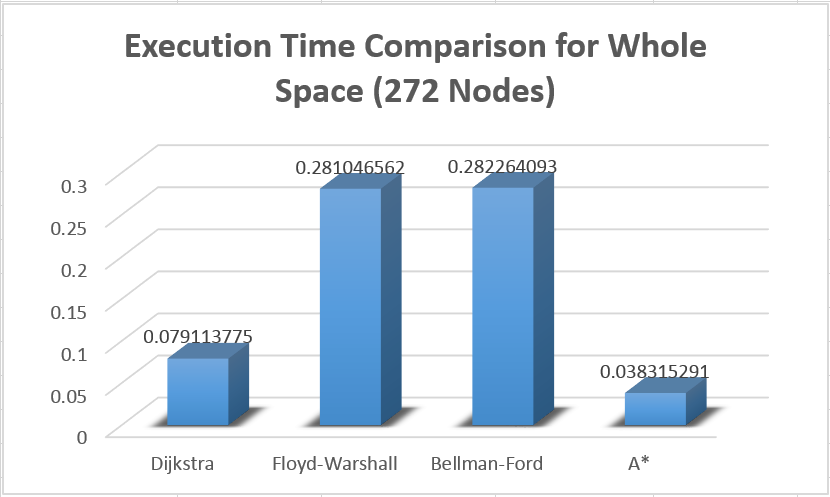
\includegraphics[scale=0.4]{graf1.PNG}
	\caption{Execution Time Comparison for Whole Space}
	\label{fig:graf1}
\end{figure}

\begin{figure}[h!]
	\centering
	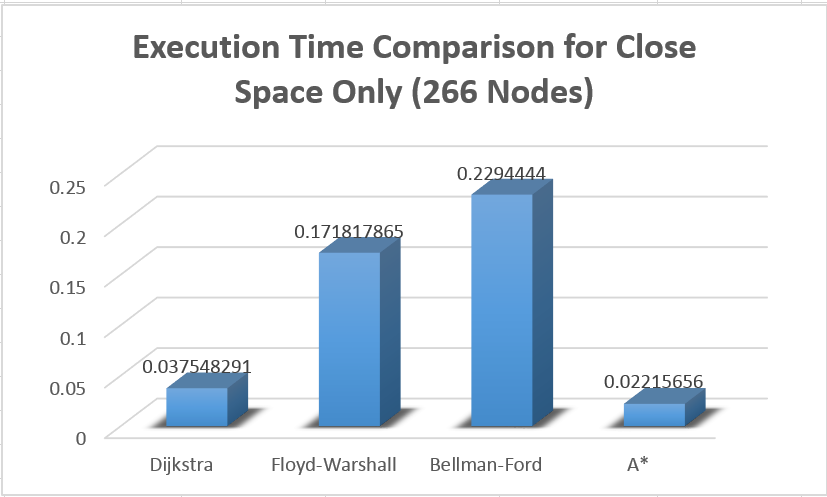
\includegraphics[scale=0.4]{graf2.PNG}
	\caption{Execution Time Comparison for Close Space Only}
	\label{fig:graf2}
\end{figure}

\begin{figure}[h!]
	\centering
	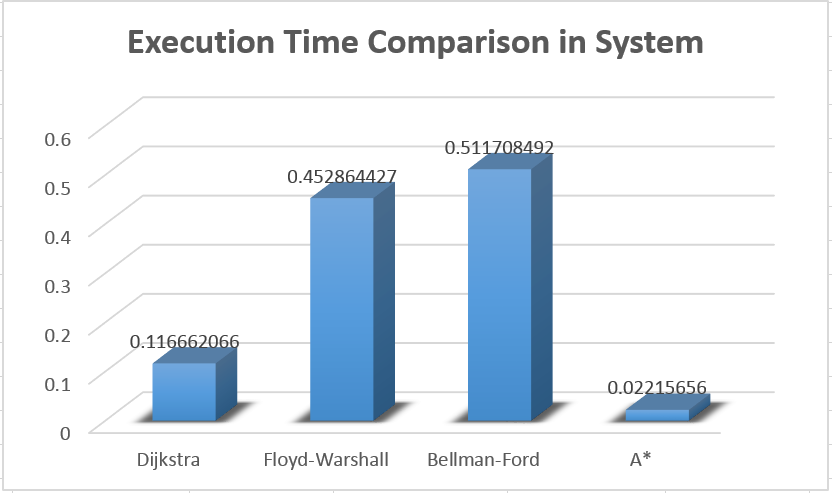
\includegraphics[scale=0.4]{graf3.PNG}
	\caption{Execution Time Comparison in System
	}
	\label{fig:graf3}
\end{figure}

\vspace{40mm}
As seen in the charts above, it could be concluded that A* Algorithm give the smallest execution time wich mean A* algorithm is the best algorithm to implement in this case besides Dijkstra, Floyd-Warshall, or Bellman-Ford algorithm. 

\subsection{Shortest Path Algorithm Testing}
This testing is about analyzing result of how each of the shortest path algorithms works, so we could know why A* can gives us the best execution time according to the previous test. The small example of graph as shown in Figure is the graph that will be used it this section to be implement in each four algorithm. Assume that the source node is node A and the destination node is node F.

\begin{figure}[h!]
	\centering
	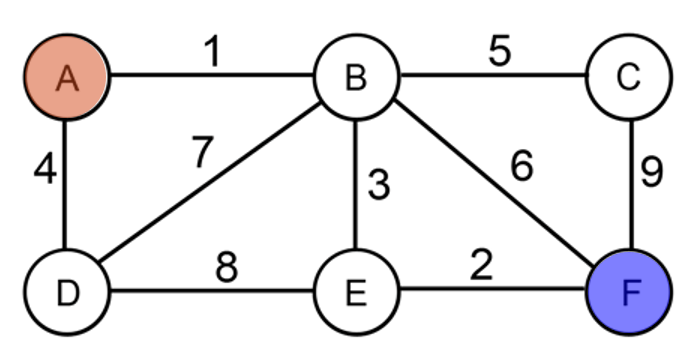
\includegraphics[scale=0.4]{figure21.png}
	\caption{Smaller graph example
	}
	\label{fig:figure21}
\end{figure}

\begin{enumerate}
	\item \textbf{Dijkstra's Algorithm}\\
	Figure \ref{fig:figure22} is the Dijkstra's Algorithm pseudocode.
	
	\begin{figure}[h!]
		\centering
		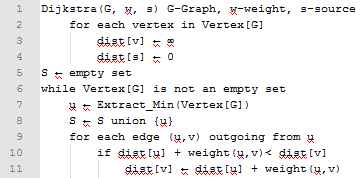
\includegraphics[scale=1]{figure6.PNG}
		\caption{Dijkstra's Algorithm pseudocode
		}
		\label{fig:figure22}
	\end{figure}

	As shown in the pseudocode, dijkstra's algorithm has two times looping of the vertex wich mean it runs in \textbf{$O(V^2)$}. Dijkstra will find the shortest path from a single source to all vertex. For the first loop, it will run until all the vertex has been accessed. And the second loop, it will check the minimum distance of its neighbours. Let's take a look to Figure \ref{table:5}
	wich is the output of dijkstra algorithm. The value in green cells are the shortest distance from node A to the nodes in orange cells.
		
% Please add the following required packages to your document preamble:
% \usepackage[table,xcdraw]{xcolor}
% If you use beamer only pass "xcolor=table" option, i.e. \documentclass[xcolor=table]{beamer}
\begin{table}[]
	\centering
	\caption{My caption}
	\label{my-label}
	\begin{tabular}{|c|r|c|c|c|c|c|c|}
		\hline
		\rowcolor[HTML]{FCFF2F} 
		\cellcolor[HTML]{C0C0C0}\textbf{Step} & \multicolumn{1}{c|}{\cellcolor[HTML]{C0C0C0}\textbf{Visited}} & \textbf{A}                         & \textbf{B}                                & \textbf{C}                                 & \textbf{D}                         & \textbf{E}                                  & \textbf{F}                                 \\ \hline
		0                                     &                                                               & 0                                  & $\infty$                                  & $\infty$                                   & $\infty$                           & $\infty$                                    & $\infty$                                   \\ \hline
		1                                     & A                                                             & 0                                  & \textbf{$\sqrt5$}                         & $\infty$                                   & 3                                  & $\infty$                                    & $\infty$                                   \\ \hline
		2                                     & A, B                                                          & 0                                  & $\sqrt5$                                  & $3\sqrt5$                                  & \textbf{3}                         & $2+\sqrt5$                                  & $3\sqrt5$                                  \\ \hline
		3                                     & A, B, D                                                       & 0                                  & $\sqrt5$                                  & $3\sqrt5$                                  & 3                                  & \textbf{$2+\sqrt5$}                         & $3\sqrt5$                                  \\ \hline
		4                                     & A, B, D, E                                                    & 0                                  & $\sqrt5$                                  & $3\sqrt5$                                  & 3                                  & $2+\sqrt5$                                  & \textbf{$3\sqrt5$}                         \\ \hline
		5                                     & A, B, D, E, F                                                 & 0                                  & $\sqrt5$                                  & \textbf{$3\sqrt5$}                         & 3                                  & $2+\sqrt5$                                  & $3\sqrt5$                                  \\ \hline
		6                                     & A, B, E, D, F, C                                              & \cellcolor[HTML]{34FF34}\textbf{0} & \cellcolor[HTML]{34FF34}\textbf{$\sqrt5$} & \cellcolor[HTML]{34FF34}\textbf{$3\sqrt5$} & \cellcolor[HTML]{34FF34}\textbf{3} & \cellcolor[HTML]{34FF34}\textbf{$2+\sqrt5$} & \cellcolor[HTML]{34FF34}\textbf{$3\sqrt5$} \\ \hline
	\end{tabular}
\end{table}
	
	\item \textbf{Floyd-Warshall Algorithm}\\
	Figure \ref{fig:figure23} is the Floyd-Warshall Algorithm pseudocode.
	
	\begin{figure}[h!]
		\centering
		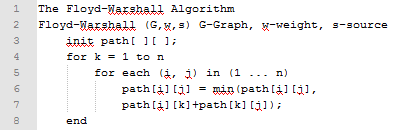
\includegraphics[scale=1]{figure7.PNG}
		\caption{Floyd-Warshall Algorithm pseudocode
		}
		\label{fig:figure23}
	\end{figure}
	
	As shown in the pseudocode, floyd-Warshall algorithm has three times looping of the vertex wich mean it runs in \textbf{$O(V^3)$}. Floyd-warshall will find the shortest path for all pairs shortest path as shown in Figure \ref{table:6} as the result of this testing case. Floyd-Warshall doesn't have any variables to save the paths. So the high time complexity and the output are the reason why this algorithm is not applicable in this Indoor Routing System.
	
	% Please add the following required packages to your document preamble:
	% \usepackage[table,xcdraw]{xcolor}
	% If you use beamer only pass "xcolor=table" option, i.e. \documentclass[xcolor=table]{beamer}
	\begin{table}[h!]
		\centering
		\caption{Floyd-Warshall Algorithm output}
		\label{table:6}
		\begin{tabular}{|
				>{\columncolor[HTML]{F8FF00}}c |c|c|c|c|c|c|}
			\hline
			& \cellcolor[HTML]{F8FF00}\textbf{A} & \cellcolor[HTML]{F8FF00}\textbf{B} & \cellcolor[HTML]{F8FF00}\textbf{C} & \cellcolor[HTML]{F8FF00}\textbf{D} & \cellcolor[HTML]{F8FF00}\textbf{E} & \cellcolor[HTML]{F8FF00}\textbf{F} \\ \hline
			\textbf{A} & 0                                  & 1                                  & 6                                  & 4                                  & 4                                  & 6                                  \\ \hline
			\textbf{B} & 1                                  & 0                                  & 5                                  & 5                                  & 3                                  & 5                                  \\ \hline
			\textbf{C} & 6                                  & 5                                  & 0                                  & 10                                 & 8                                  & 9                                  \\ \hline
			\textbf{D} & 4                                  & 5                                  & 10                                 & 0                                  & 8                                  & 10                                 \\ \hline
			\textbf{E} & 4                                  & 3                                  & 8                                  & 8                                  & 0                                  & 2                                  \\ \hline
			\textbf{F} & 6                                  & 5                                  & 9                                  & 10                                 & 2                                  & 0                                  \\ \hline
		\end{tabular}
	\end{table}
	
	\item \textbf{Bellman-Ford Algorithm}\\
	Figure \ref{fig:figure24} is the Bellman-Ford Algorithm pseudocode.
	
	\begin{figure}[h!]
		\centering
		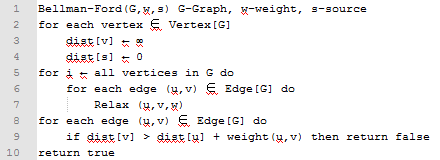
\includegraphics[scale=1]{figure8.PNG}
		\caption{Bellman-Ford Algorithm pseudocode
		}
		\label{fig:figure24}
	\end{figure}
	
	As shown in the pseudocode, Bellman-Ford algorithm has a loop to access all the vertex and a loop to access the edges, wich means it runs in \textbf{$O(VE)$}. Just like dijkstra's algorithm, bellman-ford will find the shortest path from a single source node to all nodes. The output of this algorithm for this testing case is shown in Figure \ref{table:7}. Bellman-Ford also doesn't have any variables to save the paths. So the high time complexity and the output are the reason why this algorithm is not applicable in this Indoor Routing System.
	
	% Please add the following required packages to your document preamble:
	% \usepackage[table,xcdraw]{xcolor}
	% If you use beamer only pass "xcolor=table" option, i.e. \documentclass[xcolor=table]{beamer}
	\begin{table}[h!]
		\centering
		\caption{Bellman-Ford Algorithm output}
		\label{table:7}
		\begin{tabular}{|c|c|c|c|c|c|c|}
			\hline
			\rowcolor[HTML]{F8FF00} 
			\textbf{DESTINATION} & \textbf{A} & \textbf{B} & \textbf{C} & \textbf{D} & \textbf{E} & \textbf{F} \\ \hline
			& 0          & 1          & 6          & 4          & 4          & 6          \\ \hline
		\end{tabular}
	\end{table}
	
	\item \textbf{A* Algorithm}\\
	Figure \ref{fig:figure25} is the A* Algorithm pseudocode.
	
	\begin{figure}[h!]
		\centering
		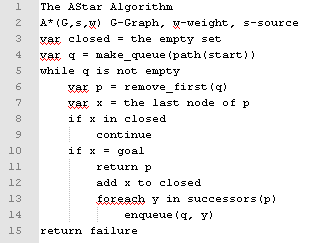
\includegraphics[scale=1]{figure9.PNG}
		\caption{A* Algorithm pseudocode
		}
		\label{fig:figure25}
	\end{figure}
	
	As shown in the pseudocode, A* algorithm has no loop wich means it runs in \textbf{$O(V)$}. A* will find the shortest path for a single source node to a single destination node as shown in Figure \ref{fig:figure25a} as the result of this testing case. A* algorithm needs the heuristic value wich is the euclidean distance between each node to the destination node. That's why the nodes' position have to be specified.
	
	\begin{figure}[h!]
		\centering
		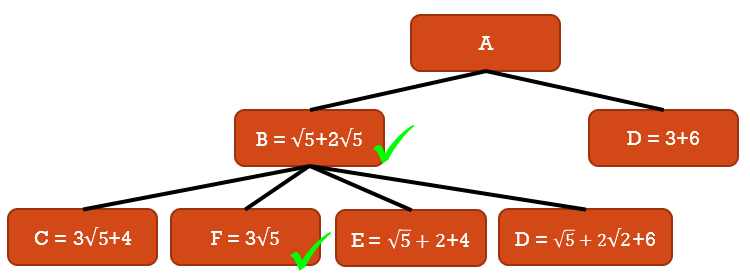
\includegraphics[scale=0.7]{figure25.PNG}
		\caption{A* Algorithm output
		}
		\label{fig:figure25a}
	\end{figure}
	\vspace{40mm}
\end{enumerate}
\subsection{Distance Calculation and Distance Measurement Testing}
Here are the result of the system's accuracy testing. This testing will show the deviation between the result of system calculation and the real distance  measurements as shown in Table \ref{table:8} and figure \ref{table:9}. All the distances are in meters.

% Please add the following required packages to your document preamble:
% \usepackage{multirow}
% \usepackage[table,xcdraw]{xcolor}
% If you use beamer only pass "xcolor=table" option, i.e. \documentclass[xcolor=table]{beamer}
\begin{table}[h!]
	\centering
	\caption{Distance deviation in shortest path search}
	\label{table:8}
	\begin{tabular}{|l|l|l|l|r|r|r|}
		\hline
		\multicolumn{1}{|c|}{}                               & \multicolumn{1}{c|}{}                                                                            & \multicolumn{1}{c|}{}                                  & \multicolumn{1}{c|}{}                                       & \multicolumn{2}{c|}{}                                                                                                                                                         & \multicolumn{1}{c|}{}                                                                                              \\
		\multicolumn{1}{|c|}{}                               & \multicolumn{1}{c|}{}                                                                            & \multicolumn{1}{c|}{}                                  & \multicolumn{1}{c|}{}                                       & \multicolumn{2}{c|}{\multirow{-2}{*}{\textbf{Shortest Distance}}}                                                                                                             & \multicolumn{1}{c|}{}                                                                                              \\ \cline{5-6}
		\multicolumn{1}{|c|}{\multirow{-3}{*}{\textbf{No.}}} & \multicolumn{1}{c|}{\multirow{-3}{*}{\textbf{Scenario}}}                                         & \multicolumn{1}{c|}{\multirow{-3}{*}{\textbf{Source}}} & \multicolumn{1}{c|}{\multirow{-3}{*}{\textbf{Destination}}} & \multicolumn{1}{c|}{\textbf{\begin{tabular}[c]{@{}c@{}}in System \\ (S)\end{tabular}}} & \multicolumn{1}{c|}{\textbf{\begin{tabular}[c]{@{}c@{}}in Real \\ (R)\end{tabular}}} & \multicolumn{1}{c|}{\multirow{-3}{*}{\textbf{\begin{tabular}[c]{@{}c@{}}Deviation \\ ($|$S - R$|$)\end{tabular}}}} \\ \hline
		1                                                    &                                                                                                  & IF3.03.04                                              & IF3.03.05                                                   & 8.661221996                                                                            & 6                                                                                    & 2.661221996                                                                                                        \\ \cline{1-1} \cline{3-7} 
		2                                                    &                                                                                                  & IF3.02.05                                              & IF3.02.01                                                   & 34.78388051                                                                            & 34.7                                                                                 & 0.083880508                                                                                                        \\ \cline{1-1} \cline{3-7} 
		3                                                    & \multirow{-3}{*}{\begin{tabular}[c]{@{}l@{}}Same\\   Building, \\ Same Z\end{tabular}}           & IF3.01.02                                              & IF3.01.03                                                   & 21.56047226                                                                            & 21.7                                                                                 & 0.139527743                                                                                                        \\ \hline
		4                                                    &                                                                                                  & IF3.03.03                                              & IF3.02.05                                                   & 38.7783564                                                                             & 34.1                                                                                 & 4.6783564                                                                                                          \\ \cline{1-1} \cline{3-7} 
		5                                                    &                                                                                                  & IF3.03.03                                              & IF3.01.05                                                   & 41.18405404                                                                            & 35.4                                                                                 & 5.784054043                                                                                                        \\ \cline{1-1} \cline{3-7} 
		6                                                    & \multirow{-3}{*}{\begin{tabular}[c]{@{}l@{}}Same\\   Building, \\ Different Z\end{tabular}}      & IF2.01.10                                              & IF2.02.09                                                   & 36.66114963                                                                            & 31                                                                                   & 5.661149626                                                                                                        \\ \hline
		7                                                    &                                                                                                  & IF2.01.05                                              & IF3.01.05                                                   & 69.19729964                                                                            & 69.3                                                                                 & 0.102700358                                                                                                        \\ \cline{1-1} \cline{3-7} 
		8                                                    &                                                                                                  & IF2.01.10                                              & IF3.01.08                                                   & 102.1953267                                                                            & 94                                                                                   & 8.195326717                                                                                                        \\ \cline{1-1} \cline{3-7} 
		9                                                    & \multirow{-3}{*}{\begin{tabular}[c]{@{}l@{}}Different\\   Building, \\ Same Z\end{tabular}}      & IF2.01.10                                              & IF1.01.01                                                   & 120.0752443                                                                            & 114.2                                                                                & 5.875244347                                                                                                        \\ \hline
		10                                                   &                                                                                                  & IF3.01.05                                              & IF2.02.05                                                   & 78.71397663                                                                            & 79.6                                                                                 & 0.886023374                                                                                                        \\ \cline{1-1} \cline{3-7} 
		11                                                   &                                                                                                  & IF2.02.01                                              & IF3.01.02                                                   & 120.9040472                                                                            & 113.1                                                                                & 7.804047212                                                                                                        \\ \cline{1-1} \cline{3-7} 
		12                                                   & \multirow{-3}{*}{\begin{tabular}[c]{@{}l@{}}Different\\   Building, \\ Different Z\end{tabular}} & IF3.03.04                                              & IF2.01.05                                                   & 87.21359285                                                                            & 87.6                                                                                 & 0.386407153                                                                                                        \\ \hline
		\rowcolor[HTML]{F8FF00} 
		\multicolumn{6}{|c|}{\cellcolor[HTML]{F8FF00}\textbf{AVERAGE}}                                                                                                                                                                                                                                                                                                                                                                                                 & \textbf{3.521495}                                                                                                  \\ \hline
	\end{tabular}
	\end{table}

% Please add the following required packages to your document preamble:
% \usepackage{multirow}
% \usepackage[table,xcdraw]{xcolor}
% If you use beamer only pass "xcolor=table" option, i.e. \documentclass[xcolor=table]{beamer}
\begin{table}[h!]
	\centering
	\caption{Distance deviation in closed shortest path search}
	\label{table:9}
	\begin{tabular}{|l|l|l|l|r|r|r|}
		\hline
		\multicolumn{1}{|c|}{}                               & \multicolumn{1}{c|}{}                                                                            & \multicolumn{1}{c|}{}                                  & \multicolumn{1}{c|}{}                                       & \multicolumn{2}{c|}{}                                                                                                                                                         & \multicolumn{1}{c|}{}                                                                                              \\
		\multicolumn{1}{|c|}{}                               & \multicolumn{1}{c|}{}                                                                            & \multicolumn{1}{c|}{}                                  & \multicolumn{1}{c|}{}                                       & \multicolumn{2}{c|}{\multirow{-2}{*}{\textbf{Shortest Distance}}}                                                                                                             & \multicolumn{1}{c|}{}                                                                                              \\ \cline{5-6}
		\multicolumn{1}{|c|}{\multirow{-3}{*}{\textbf{No.}}} & \multicolumn{1}{c|}{\multirow{-3}{*}{\textbf{Scenario}}}                                         & \multicolumn{1}{c|}{\multirow{-3}{*}{\textbf{Source}}} & \multicolumn{1}{c|}{\multirow{-3}{*}{\textbf{Destination}}} & \multicolumn{1}{c|}{\textbf{\begin{tabular}[c]{@{}c@{}}in System \\ (S)\end{tabular}}} & \multicolumn{1}{c|}{\textbf{\begin{tabular}[c]{@{}c@{}}in Real \\ (R)\end{tabular}}} & \multicolumn{1}{c|}{\multirow{-3}{*}{\textbf{\begin{tabular}[c]{@{}c@{}}Deviation \\ ($|$S - R$|$)\end{tabular}}}} \\ \hline
		1                                                    &                                                                                                  & IF3.03.04                                              & IF3.03.05                                                   & 8.661221996                                                                            & 6                                                                                    & 2.661221996                                                                                                        \\ \cline{1-1} \cline{3-7} 
		2                                                    &                                                                                                  & IF3.02.05                                              & IF3.02.01                                                   & 34.78388051                                                                            & 34.7                                                                                 & 0.083880508                                                                                                        \\ \cline{1-1} \cline{3-7} 
		3                                                    & \multirow{-3}{*}{\begin{tabular}[c]{@{}l@{}}Same\\   Building, \\ Same Z\end{tabular}}           & IF3.01.02                                              & IF3.01.03                                                   & 21.56047226                                                                            & 21.7                                                                                 & 0.139527743                                                                                                        \\ \hline
		4                                                    &                                                                                                  & IF3.03.03                                              & IF3.02.05                                                   & 38.7783564                                                                             & 34.1                                                                                 & 4.6783564                                                                                                          \\ \cline{1-1} \cline{3-7} 
		5                                                    &                                                                                                  & IF3.03.03                                              & IF3.01.05                                                   & 41.18405404                                                                            & 35.4                                                                                 & 5.784054043                                                                                                        \\ \cline{1-1} \cline{3-7} 
		6                                                    & \multirow{-3}{*}{\begin{tabular}[c]{@{}l@{}}Same\\   Building, \\ Different Z\end{tabular}}      & IF2.01.10                                              & IF2.02.09                                                   & 36.66114963                                                                            & 31                                                                                   & 5.661149626                                                                                                        \\ \hline
		7                                                    &                                                                                                  & IF2.01.05                                              & IF3.01.05                                                   & 168.010905                                                                             & 168.8                                                                                & 0.789095019                                                                                                        \\ \cline{1-1} \cline{3-7} 
		8                                                    &                                                                                                  & IF2.01.10                                              & IF3.01.08                                                   & 102.1953267                                                                            & 94                                                                                   & 8.195326717                                                                                                        \\ \cline{1-1} \cline{3-7} 
		9                                                    & \multirow{-3}{*}{\begin{tabular}[c]{@{}l@{}}Different\\   Building, \\ Same Z\end{tabular}}      & IF2.01.10                                              & IF1.01.01                                                   & 140.9867135                                                                            & 135.5                                                                                & 5.48671352                                                                                                         \\ \hline
		10                                                   &                                                                                                  & IF3.01.05                                              & IF2.02.05                                                   & 177.5121245                                                                            & 177.8                                                                                & 0.287875482                                                                                                        \\ \cline{1-1} \cline{3-7} 
		11                                                   &                                                                                                  & IF2.02.01                                              & IF3.01.02                                                   & 234.2925391                                                                            & 234.6                                                                                & 0.307460939                                                                                                        \\ \cline{1-1} \cline{3-7} 
		12                                                   & \multirow{-3}{*}{\begin{tabular}[c]{@{}l@{}}Different\\   Building, \\ Different Z\end{tabular}} & IF3.03.04                                              & IF2.01.05                                                   & 187.8782596                                                                            & 184.8                                                                                & 3.07825964                                                                                                         \\ \hline
		\rowcolor[HTML]{F8FF00} 
		\multicolumn{6}{|c|}{\cellcolor[HTML]{F8FF00}\textbf{AVERAGE}}                                                                                                                                                                                                                                                                                                                                                                                                 & \textbf{3.096076803}                                                                                               \\ \hline
	\end{tabular}
\end{table}

\vspace{60mm}
Figure \ref{fig:graf3} and \ref{fig:graf8} shows the fluctuation of the testing deviation result. From the chart, we can see that the daviation result is quiet fluctuate. This result means that this system has a deficiency in resuting the distance with average deviation velue is 4.543359576 meters.


\begin{figure}[h!]
	\centering
	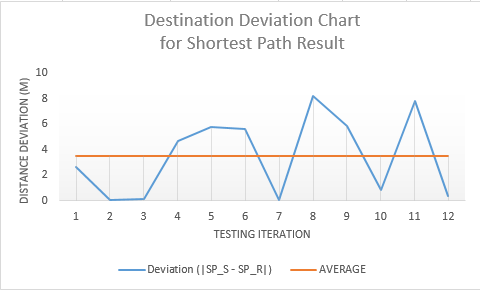
\includegraphics[scale=1]{graf4.PNG}
	\caption{Distance deviation testing result for shortest path
	}
	\label{fig:graf3}
\end{figure}

\begin{figure}[h!]
	\centering
	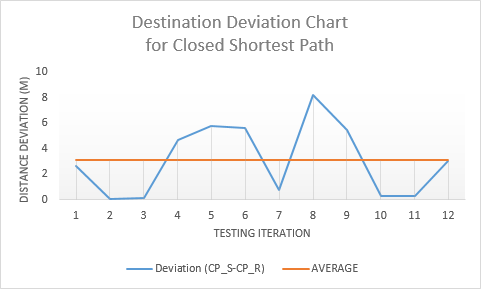
\includegraphics[scale=1]{graf5.PNG}
	\caption{Distance deviation testing result for close shortest path
	}
	\label{fig:graf8}
\end{figure}

\vspace{30mm}
\section{Summary}
This chapter shows us the testing and analyzing result of this final project. The components that will be the testing objects are the shortest path algorithms' work, the execution time comparison between the shortest path algorithm, and also thee comparison between system's shortest distance and the shortest distance in real life. And after all the testing and analyzing process have done, it giving us a result that is A* algorithm is the most applicable and efficient to implement in this indoor routing system because it has the lowest value of execution time and the time complexity between Dijkstra's, Floyd-Warshall, and Bellman-Ford algorithms.
